\documentclass[lighthipster]{simplehipstercv}

% available options are: darkhipster, lighthipster, pastel, allblack, grey, verylight, withoutsidebar
% withoutsidebar
\usepackage[utf8]{inputenc}
\usepackage[default]{raleway}
\usepackage[margin=1cm, a4paper]{geometry}
\usepackage{enumitem}
\usepackage{fontawesome}
\usepackage{tikz}
\usepackage{graphicx}
\usepackage{xcolor}
%\usepackage{fontspec}

\usepackage{silence}
% Masque l'avertissement spécifique à la substitution de police Font Awesome
\WarningFilter{latexfont}{Font shape 'U/fontawesometwo/regular/n' undefined}
\WarningFilter{latexfont}{Font shape 'U/fontawesometwo/m/sl' undefined}
\WarningFilter{latexfont}{Font shape 'U/fontawesometwo/regular/sl' undefined}
\WarningFilter{latexfont}{Some font shapes were not available, defaults substituted}
\WarningFilter{latexfont}{Font shape 'U/fontawesometwo/regular/n' undefined}
\WarningFilter{latexfont}{Some font shapes were not available, defaults substituted}

\makeatletter
% Redirige le message d'avertissement de substitution de police
\def\f@ntas@warn#1{%
  \immediate\write\@auxout{%
    \string\GenericWarning{(#1)}{%
      LaTeX Font Warning: Font shape `U/fontawesometwo/regular/n' undefined\MessageBreak
      (Font) using `U/fontawesometwo/m/n' instead%
    }%
  }%
}
\makeatother

% a mashup of hipstercv, friggeri and twenty cv
% https://www.latextemplates.com/template/twenty-seconds-resumecv
% https://www.latextemplates.com/template/friggeri-resume-cv

%------------------------------------------------------------------ Variablen

\newlength{\rightcolwidth}
\newlength{\leftcolwidth}
\setlength{\leftcolwidth}{0.23\textwidth}
\setlength{\rightcolwidth}{0.75\textwidth}


%------------------------------------------------------------------
\title{Mary Ammar CV}
\author{\LaTeX{} Ninja}
\date{October 2025}

\pagestyle{empty}
\begin{document}

    
\thispagestyle{empty}
%-------------------------------------------------------------

\section*{Start}

\simpleheader{headercolour}{Mary}{Ammar}{Data Scientist}{white}



%------------------------------------------------

% this has to be here so the paracols starts..
\subsection*{}
\vspace{4em}

\setlength{\columnsep}{1.5cm}
\columnratio{0.25}
\begin{paracol}{2}
\raggedright % <--- Essentiel
\hbadness5000 % <--- Utile pour les petites erreurs de coupure
%\backgroundcolor{c[1]}[rgb]{1,1,0.8} % cream yellow for column-1 %\backgroundcolor{g}[rgb]{0.8,1,1} % \backgroundcolor{l}[rgb]{0,0,0.7} % dark blue for left margin




\paracolbackgroundoptions

% 0.9,0.9,0.9 -- 0.8,0.8,0.8


\footnotesize
{\setasidefontcolour
\flushright

\begin{center}
\begin{tikzpicture}
  \clip (0,0) circle (2cm);
  \node at (0,-0.8) {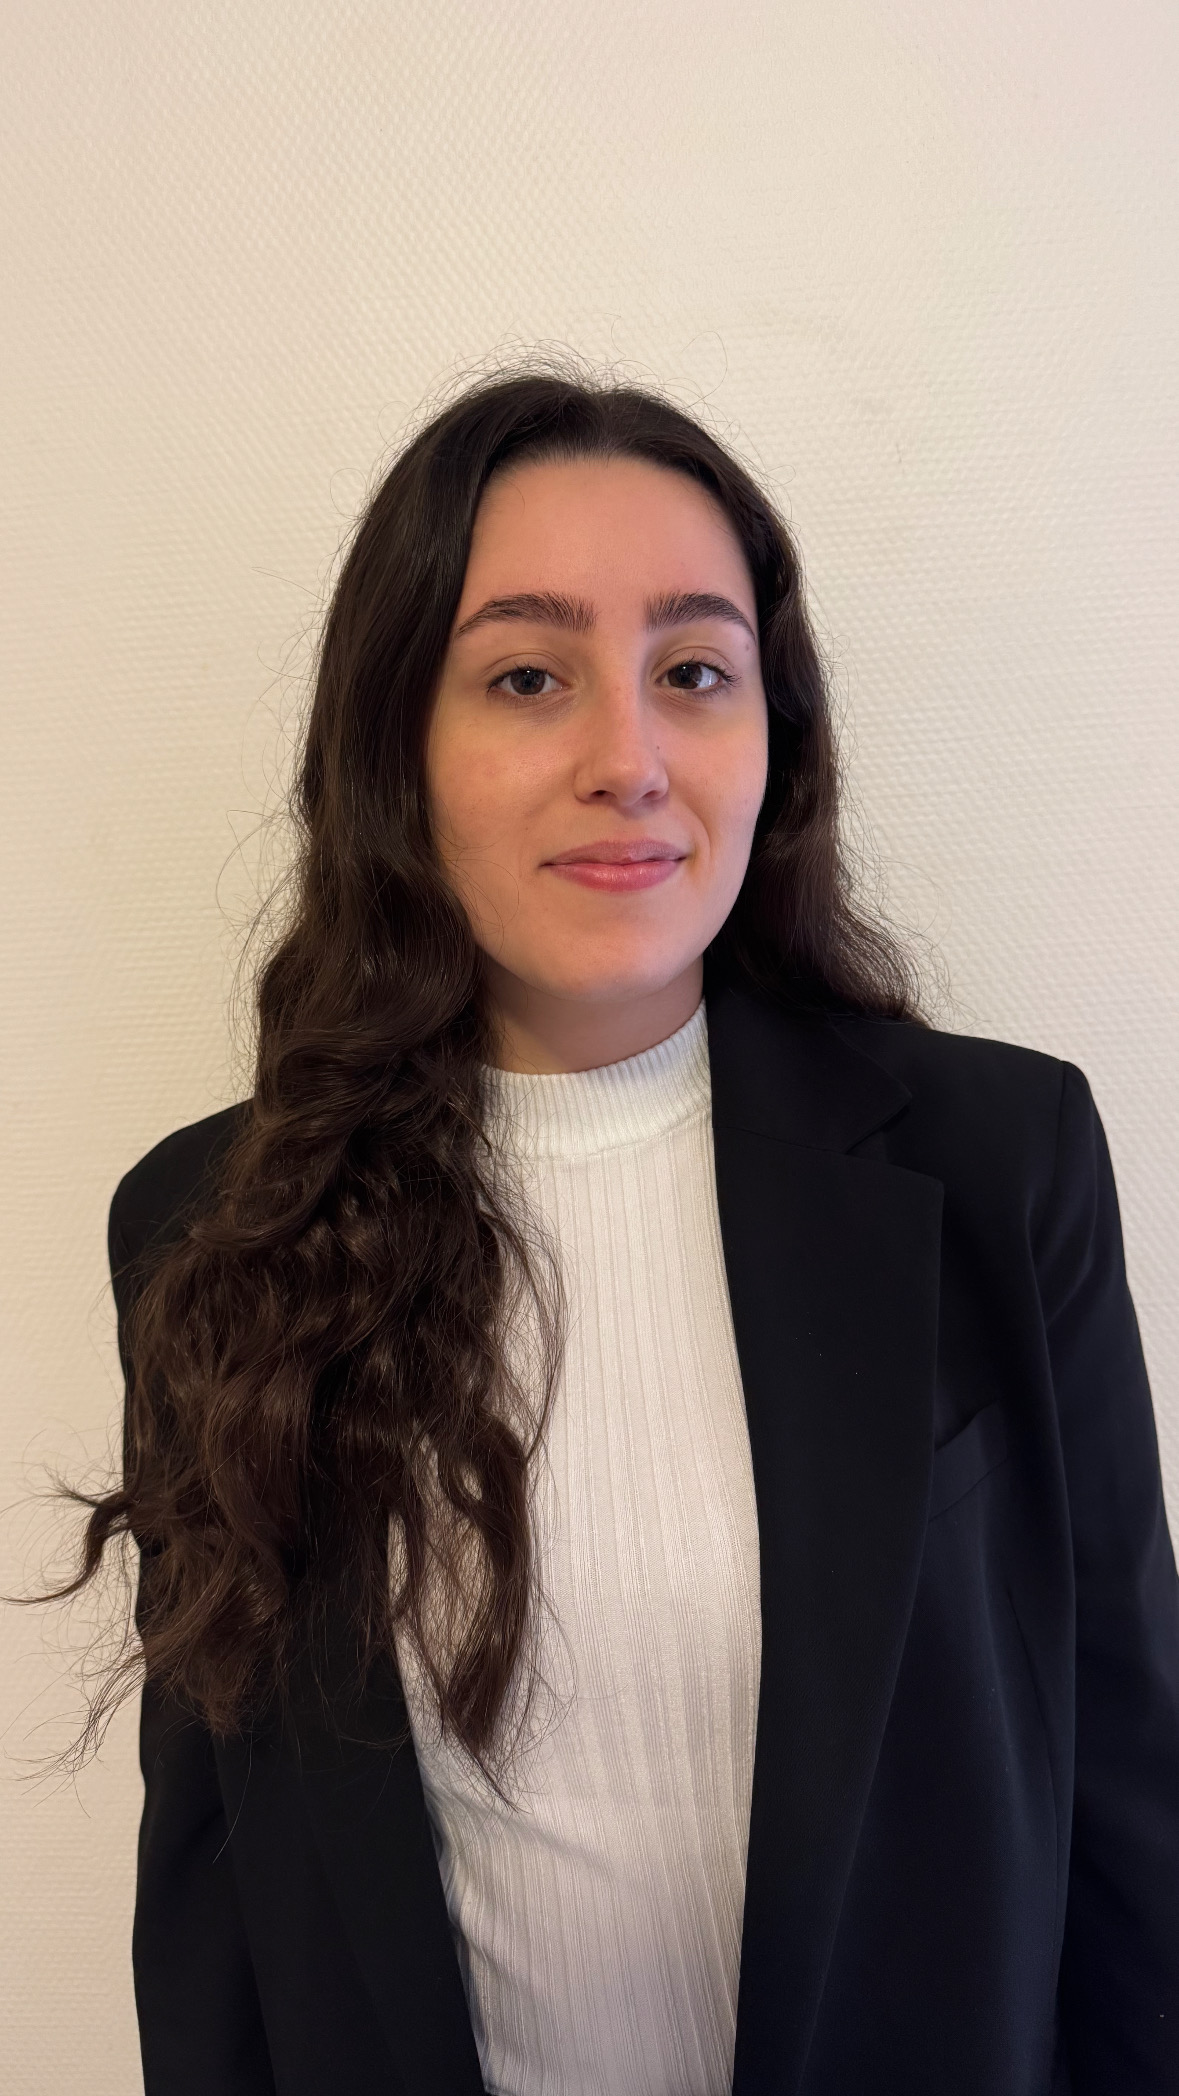
\includegraphics[width=4.5cm]{Mary.JPG}}; % ↓ descend l’image
  \draw[line width=0.6pt, color=gray] (0,0) circle (2cm);
\end{tikzpicture}
\end{center}

\bg{cvgreen}{white}{About me}\\[0.5em]

{{\footnotesize
Master's student in Scientific Computing, passionate about data analysis, modeling, and innovation.  
Curious and motivated to apply mathematical and computational tools to real-world problems.
}
}
\bigskip

\bg{cvgreen}{white}{Personal} \\[0.5em]
Mary Ammar

Nationality: Lebanese 

2002

\bigskip


\bg{cvgreen}{white}{Interests}\\[0.5em]
Data Science\\
Machine Learning\\
Travel\\
Music\\


\vspace{4em}

%\infobubble{\faTwitter}{cvgreen}{white}{@sparrow}
%\infobubble{\faFacebook}{cvgreen}{white}{}
\icon{\faGithub}{cvgreen}{white}{\href{https://github.com/mary-ammar-univ}{mary-ammar-univ}}
\icon{\faLinkedin}{cvgreen}{white}{\href{https://www.linkedin.com/in/mary-ammar-45b987267}{Mary Ammar}}

\phantom{turn the page}

\phantom{turn the page}
}
%-----------------------------------------------------------
\switchcolumn

\small
\section*{Professional Experience}

\textbf{Feb 2025 -- Aug 2025} \hfill \textbf{B2A Laboratory, Strasbourg, France}\\
\textit{Data Science Intern}
\begin{itemize}[leftmargin=2em, itemsep=0.2em, topsep=0em]
    \item Used SQL to extract and manage data from the Laboratory Information System (LIS).
    \item Processed and analyzed complex real-world datasets using R (data cleaning, structuring, and exploratory analysis).
    \item Collaborated with medical researchers to translate business needs into data-driven insights.
    \item Created clear and interactive visualizations using \texttt{ggplot2} and \texttt{plotly}.
    \item Developed an RShiny dashboard used by researchers to monitor and analyze STI results.
    \item Wrote analytical reports and presented results to the research team.
\end{itemize}

\textbf{Apr 2024 -- Jun 2024} \hfill \textbf{Institute of Molecular Plant Biology (IBMP), Strasbourg, France}\\
\textit{Data Analyst Intern}
\begin{itemize}[leftmargin=2em, itemsep=0.2em, topsep=0em]
    \item Performed Principal Component Analysis (PCA) on plant RNA datasets using R.
    \item Applied statistical tests (Student, ANOVA, Kruskal–Wallis, Wilcoxon) to compare genetic variations between wild-type and mutant strains.
    \item Generated visual summaries and statistical interpretations for research insights.
    \item Used version control tools such as Git for collaborative work and reproducibility.
\end{itemize}

\vspace{-0.5em}


\section*{Education}

\textbf{2025 -- Present} \hfill \textbf{University of Strasbourg, France}\\
\textit{Master’s Degree in Scientific Computing and Mathematics for Innovation (CSMI)}
\begin{itemize}[leftmargin=2em, itemsep=0.2em, topsep=0em]
    \item Focus on numerical analysis, mathematical modeling, optimization, and applied data science.
    \item Coursework includes high-performance computing, simulation, and machine learning.
    \item Development of computational tools for scientific innovation and real-world problem solving.
\end{itemize}

\textbf{2023 -- 2025} \hfill \textbf{University of Strasbourg, France}\\
\textit{Master’s Degree in Statistics}
\begin{itemize}[leftmargin=2em, itemsep=0.2em, topsep=0em]
    \item Machine Learning and Neural Networks: NumPy, Pandas, Scikit-Learn, TensorFlow, PyTorch, Keras.
    \item Advanced Data Analysis: PCA, CA, MCA, Cluster Analysis, and Descriptive Statistics.
    \item Bayesian Statistics and Generalized Linear Models (GLMs).
    \item Survival and Reliability Analysis, Quality Control, and Risk Modeling.
    \item Programming and Statistical Tools: R, Python, SAS.
\end{itemize}

\textbf{2020 -- 2023} \hfill \textbf{University of Strasbourg, France}\\
\textit{Bachelor’s Degree in Applied Mathematics}
\begin{itemize}[leftmargin=2em, itemsep=0.2em, topsep=0em]
    \item Studied advanced statistics, probability theory, and numerical analysis.
    \item Applied mathematical models to real-world problems.
    \item Programming in C++: data structures, algorithms, and numerical computation.
\end{itemize}

\textbf{2019 -- 2020} \hfill \textbf{Official High School of Antelias, Lebanon}\\
\textit{Scientific Baccalaureate}
\begin{itemize}[leftmargin=2em, itemsep=0.2em, topsep=0em]
    \item Specialized in mathematics, physics, and experimental sciences.
    \item Graduated with distinction in scientific subjects.
\end{itemize}




\vspace{1em}

\begin{minipage}[t]{0.28\linewidth}
\setlength{\hfuzz}{100pt} % Tolérance extrême (plus que nécessaire)
\tolerance=9999          % Autorise les très mauvaises coupures (force la ligne à tenir)
\emergencystretch=1em    % Ajoute de l'espace si nécessaire pour faire tenir la ligne
\section*{Languages}
\begin{tabular}{l | ll}
\textbf{Arabic} & C1 & {\phantom{x}\footnotesize mother tongue} \\
\textbf{French} & B2 & \pictofraction{\faCircle}{cvgreen}{4}{black!30}{3}{\tiny} \\
\textbf{English} & B2 & \pictofraction{\faCircle}{cvgreen}{4}{black!30}{3}{\tiny} %\\
%\textbf{Italian} & C2 & \pictofraction{\faCircle}{cvgreen}{3}{black!30}{1}{\tiny}
\end{tabular}
\end{minipage}\hfill
\begin{minipage}[t]{0.3\linewidth}
\setlength{\hfuzz}{100pt} % Tolérance extrême (plus que nécessaire)
\tolerance=9999          % Autorise les très mauvaises coupures (force la ligne à tenir)
\emergencystretch=1em    % Ajoute de l'espace si nécessaire pour faire tenir la ligne
\section*{Programming}
\begin{tabular}{r @{\hspace{0.5em}}l}
     \bg{skilllabelcolour}{iconcolour}{Python, R}& \barrule{0.55}{0.5em}{cvgreen} \\
     \bg{skilllabelcolour}{iconcolour}{\LaTeX} & \barrule{0.55}{0.5em}{cvgreen} \\
     \bg{skilllabelcolour}{iconcolour}{SAS} & \barrule{0.5}{0.5em}{cvpurple} \\
     \bg{skilllabelcolour}{iconcolour}{C,C++} & \barrule{0.25}{0.5em}{cvpurple} \\
\end{tabular}
\end{minipage}






\vfill{} % Whitespace before final footer

%----------------------------------------------------------------------------------------
%	FINAL FOOTER
%----------------------------------------------------------------------------------------
\setlength{\parindent}{0pt}
\begin{minipage}[t]{\linewidth}
    
\begin{center}\fontfamily{\sfdefault}\selectfont \color{black!70}
{\small Mary Ammar\icon{\faEnvelopeO}{cvgreen}{} ammarmary02@gmail.com\icon{\faMapMarker}{cvgreen}{} Strasbourg \icon{\faPhone}{cvgreen}{} 07 32 69 41 65 %\newline\icon{\faAt}{cvgreen}{} \protect\url{jack@sparrow.com}
}
\end{center}
\end{minipage}

\end{paracol}

\end{document}